% \documentclass[a4paper,11pt]{article}
% \usepackage[hyperref]{beamerarticle}

\documentclass[final]{beamer}

\usepackage[hangul]{kotex}
\usepackage{amsfonts,amsmath,xob-amssymb}

\usepackage{amsthm}
\newtheorem{defn}{Definition}
\newtheorem{thm}{Theorem}

\usepackage{cancel}
\graphicspath{{./_img/03/}}

\usepackage{graphicx}
\usepackage{media9}
\usepackage{tikz}
\usepackage{textpos}

\mode<presentation>{
	\usetheme{Madrid}
	\usecolortheme{default}
	\usefonttheme{professionalfonts}
}

\def\b{\boldsymbol}

\mode<article>{
\usepackage{fullpage}
}
\usepackage{ulem}

\newcommand{\bb}{\mathbb}
\newcommand{\bd}{\mathbf}
\newcommand{\p}{\partial}

\newcounter{saveenumi}
\newcommand{\seti}{\setcounter{saveenumi}{\value{enumi}}}
\newcommand{\conti}{\setcounter{enumi}{\value{saveenumi}}}

\newcommand{\mail}{\url{mailto:experiment.namun+2016f@gmail.com} }


\title{게임이론 Part 1}
\subtitle{게임의 기본 개념들 (게임이론, 진화, 그리고 협력)}
\author[조남운]{허준석$\rightarrow$이동한$\rightarrow$\emph{조남운}\\\mail}

\begin{document}

\begin{frame}[t]{title}
	\titlepage
\end{frame}
%--- Next Frame ---%

\begin{frame}[t]{목차}
	\tableofcontents
\end{frame}
%--- Next Frame ---%

\section{게임의 구성요소} % (fold)
\label{sec:basicStructure}
\begin{frame}[t]{게임의 4가지 구성요소}
	\begin{enumerate}
		\item 참가자 (Players, or Participants)
		\item 전략 (Actions, or Strategies)
		\item 결과 (Outcomes)
		\item 보수 (Payoffs)
	\end{enumerate}
	\begin{center}
	\fbox{\includegraphics[height=.4\textheight]{gamejam.png}}
	\end{center}
\end{frame}
%--- Next Frame ---%

\begin{frame}[t]{Players}
	\begin{columns}[c]
		\column{.6\textwidth}
		\begin{itemize}
			\item 선수들은 2명 이상 (일반적으로 $N$ 명)
			\item 선수들은 `합리적'이라고 가정 (economic rationality)
			\item 여기서 합리적이란 두가지 의미 
			\begin{enumerate}
				\item 각자 자신의 이득을 극대화한다. 
				\item common knowledge 
			\end{enumerate}
		\end{itemize}
		\column{.4\textwidth}
		\fbox{\includegraphics[width=.8\textwidth]{Sofonisba.jpg}}
	\end{columns}
\end{frame}
%--- Next Frame ---%

\begin{frame}[t]{Common Knowledge}
	\begin{itemize}
		\item 논리학 용어로 ``상식''과는 다른 의미
		\item 게임 참가자들에 대한 특별한 종류의 지식구조
	\end{itemize}
	\begin{center}
		\framebox[\textwidth]{
		\begin{quote}\ttfamily
			어떤 집단의 선수들이 $p$라는 내용을 을 알고 있다. 이들은 모두가 $p$를 알고 있다는 사실을 알고 있고, 이 사실($p$를 알고 있다는 사실을 알고 있다는 사실)을 알고 있다는 것을 알고 있고... 
		\end{quote}
		}
	\end{center}
\end{frame}
%--- Next Frame ---%

\begin{frame}[t]{모자를 쓴 아이}
	\begin{columns}
		\column{.7\textwidth}
		\begin{itemize}
			\item 아이 3명이 서로 마주보고 있다 (아이1, 아이2, 아이3)
			\item 각 아이들은 빨간색 모자를 쓰고 있거나 흰색 모자를 쓰고 있다
			\item 각 아이들은 다른 아이들의 모자 색을 볼 수 있지만, 자기가 쓴 모자의 색은 볼 수 없다. 
			\item (일단 아이들이 쓰고 있는 모자가 모두 빨간 색이라고 가정하자)
			\item 교사가 들어와 자기가 쓴 모자의 색을 알겠는지 물어본다. 
		\end{itemize}
		\column{.3\textwidth}
		\fbox{\includegraphics[width=.8\textwidth]{redhat.png}}
	\end{columns}
\end{frame}
%--- Next Frame ---%

\begin{frame}[t]{모자를 쓴 아이 (계속)}
	\begin{itemize}
		\item 이제 선생님이 다시 이렇게 말한다. \\[1em] {\color{red}{\hspace{2em}``적어도 한 명은 빨간 색 모자를 쓰고 있다!''}}
		\vspace{1em}
		\item 이제 아이 1,2,3이 차례로 답한다. 
		\item 아이 1의 대답은? ``잘 모르겠다.''
		\item 아이 2의 대답은? ``잘 모르겠다."
		\item 아이 3의 대답은? ``알겠다! 나는 빨간색 모자를 쓰고 있다!''
	\end{itemize}
\end{frame}
%--- Next Frame ---%

\begin{frame}[t]{Common Knowledge}
	\begin{columns}[c]
		\column{.6\textwidth}
		\begin{itemize}
			\item 만일 소녀 2,3의 모자가 모두 흰색이었다면 소녀 1의 답은?
			\item 만일 소녀 3의 모자가 흰색이었다면 소녀 2의 대답은?
			\item 그래서, 소녀 3은 자신이 빨간 모자를 써다는 점을 알 수 있다!
		\end{itemize}
		\column{.4\textwidth}
		\fbox{\includegraphics[width=.8\textwidth]{miracle.png}}
	\end{columns}
\end{frame}
%--- Next Frame ---%

\begin{frame}[t]{Common Knowledge (계속)}
	\begin{itemize}
		\item 어떻게 세번째 소녀는 자신의 모자 색을 맞출 수 있었는가?
		\item Common Knowledges (CKs)
		\begin{enumerate}[CK1]
			\item 교사가 공표한 사실 (최소 1명은 빨간모자 쓰고 있다)
			\item 위 공표한 사실을 모두가 알고 있다는 사실
			\item 이 사실을 모두가 알고 있기 때문에 내릴 수 있는 결론을 알고 있다는 사실
		\end{enumerate}
		\item 하지만, 아이1이나 아이2가 가령 확실히 알 수 있는 상황(대답하지 않은 아이들이 모두 흰색모자를 쓴 상황)에서도 잘 모르겠다고 대답했다면? 
		\begin{itemize}
			\item CK3 위배 - 이 사실을 모르는 아이3의 추론은 틀릴 수 있게 됨
		\end{itemize}
	\end{itemize}
\end{frame}
%--- Next Frame ---%

\begin{frame}[t]{Strong Rationality}
	\begin{columns}[c]
		\column{.6\textwidth}
		\begin{itemize}
			\item 게임이론은 `균형'을 탐구
			\item 균형이 계산가능하게 되기 위한 전제들
			\begin{itemize}
				\item 사람들은 자신의 이익을 극대화한다
				\item 이를 위해 사람들은 자신이 지닌 정보를 최대한 논리적으로 활용한다
			\end{itemize}
			\item 현실에서 사람들은 정말로 이렇게 추론할까?
			\item 위 가정들은 굉장히 강한 가정이라는 점을 염두에 둬야함
		\end{itemize}
		\column{.4\textwidth}
		\fbox{\includegraphics[width=.8\textwidth]{equilibrium.jpg}}
	\end{columns}
\end{frame}
%--- Next Frame ---%

\begin{frame}[t]{Actions, or Strategies}
	\begin{itemize}
		\item Action: 현 상황에서 내가 취할 수 있는 행동의 집합
		\item Strategy: ``사전적''으로 정의되는 가능한 모든 상황들에 대한 Action Plan
		\item 게임 플레이 전에 가능한 모든 상황에 대해 검토하고 결론을 내려둬야 함
		\item 실제 플레이: ult1, ult2
	\end{itemize}
\end{frame}
%--- Next Frame ---%

\begin{frame}[t]{Strategic Ultimatum Game}
	\begin{itemize}
		\item 실제로 해보자!
		\item Phase I: 단순 ultimatum game 3회 실시
		\item Phase II: ultimatum game version2 : strategic form
		\begin{itemize}
			\item 제안자(Proposer)는 동일
			\item 수용자(Responder)는 제안자의 전략을 알지 못하는 상태에서 자신이 제안받을 수 있는 모든 경우에 대해서 응답을 설정함
		\end{itemize}
	\end{itemize}
\end{frame}
%--- Next Frame ---%

\begin{frame}[t]{Strategy}
	\begin{itemize}
		\item 단 한 번 하는 죄수의 딜레마라면?
		\item 만일 동일 상대와 죄수의 딜레마를 3회에 걸쳐서 한다면?
		\item 이 게임을 시작하기 전에 나의 게임 플랜은? 
		\item 이렇게 게임을 시작하기 전에 정의하는 것이 전략
	\end{itemize}
\end{frame}
%--- Next Frame ---%

\begin{frame}[t]{Strategy (Example)}
	\begin{itemize}
		\item 타자가 타석에 들어섰다. 투수가 제1구를 던졌다. (타자는 타구를 읽을 수 있는 것으로 가정)
		\item 타자의 전략?
		\begin{itemize}
			\item ``직구면 크게 휘두른다!'' 만으로는 전략이 되지 않음
		\end{itemize}
		\item 타자의 전략 (완전한 버젼)
		\begin{itemize}
			\item 직구일 경우 크게 휘두름
			\item 변화구일 경우 밀어 침
			\item $\cdots$
			\item ((모든 가능성에 대해서 Action이 정해져 있어야 함))
		\end{itemize}
	\end{itemize}
\end{frame}
%--- Next Frame ---%

\begin{frame}[t]{죄수의 딜레마 다시 보기}
	\begin{columns}[c]
		\column{15em}
		\begin{center}
		\begin{table}
			\setlength{\tabcolsep}{1.2em}
			\begin{tabular}{|c|c|c|} \hline
				& {C} &  {D}\\ \hline
				{C} & {$R$}, {$R$} & {$S$}, {$T$} \\ \hline%
				{D} & {$T$}, {$S$}  & {$P$}, {$P$} \\ 
				\hline
			\end{tabular}
		\end{table}
		\end{center}
		\column{15em}
		\begin{enumerate}
			\item 선수는? 
			\item 선수들의 전략은? 
			\item 결과는? 
			\item 보수는?
		\end{enumerate}
	\end{columns}
\end{frame}
%--- Next Frame ---%
% section basicStructure (end)

\section{Equilibrium} % (fold)
\label{sec:equilibrium}

\begin{frame}[t]{게임이론에서의 균형}
	\begin{columns}[c]
		\column{18em}
		\begin{itemize}
			\item 게임이론의 강점은 문제/갈등의 구조를 서술하는 데 있지 않고 
			\item 그 구조에서 어떤 결과나 나올 것인지를 예측하는 데 있음
			\item 따라서 균형 개념이 몹시 중요
		\end{itemize}
		\column{13em}
		\fbox{\includegraphics[width=12.5em]{bimbokind.jpg}}
	\end{columns}
\end{frame}
%--- Next Frame ---%

\begin{frame}[t]{강우월전략(Strong Dominant Strategy}
	\begin{columns}[c]
		\column{18em}
		\begin{itemize}
			\item 강우월전략이란 상대의 선택과 관계없이 나에게 항상 높은 보수를 보장하는 전략
			\item 일단 ``높은''이라는 말의 의미는 {\color{red}{$\geq$}}가 아닌 {\color{red}{$>$}}임 \\
		그래서 ``강强우월전략''이라고 정의
		\end{itemize}
		\column{13em}
		\fbox{\includegraphics[width=12.5em]{tilted.jpg}}
	\end{columns}
\end{frame}
%--- Next Frame ---%

\begin{frame}[t]{우월전략을 통한 균형 찾기}
	\begin{itemize}
		\item 일단, 나는 상대의 눈치를 볼 필요가 없이 전략을 결정하고 
		\item 다른 모든 플레어어도 마찬가지라면 강우월 전략이 균형일 수 있음
		\item 앞서 배웠던 CK (Common Knowledge)를 이용해서 균형을 찾아본다면? 
	\end{itemize}
\end{frame}
%--- Next Frame ---%

\begin{frame}[t]{열등전략을 지워나가기}
	\begin{center}
	\begin{table}
	\setlength{\tabcolsep}{1.2em}
	\begin{tabular}{|c|c|c|} \hline
	& {C} &  {D}\\ \hline
	{C} & {$R$}, {$R$} & {$S$}, {$T$} \\ \hline%
	{D} & {$T$}, {$S$}  & {$P$}, {$P$} \\ 
	\hline
	\end{tabular}
	\end{table}
	\end{center}

	\pause
	\begin{textblock*}{5cm}[1,1](80mm, -13mm)%
	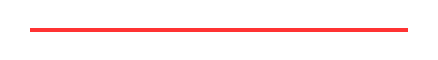
\begin{tikzpicture}
	\draw[red!80,ultra thick] (0,0) --(4.8,0);
	\end{tikzpicture}
	\end{textblock*}

	\pause
	\begin{textblock*}{5cm}[1,1](102mm, 0mm)%
	
\begin{tikzpicture}
	\draw[red!80,ultra thick] (0,0) --(0,2.5);
	\end{tikzpicture}
	\end{textblock*}

	\vspace{2em}

	\begin{center}
	\begin{table}
	\setlength{\tabcolsep}{1.2em}
	\begin{tabular}{|c|c|c|} \hline
	& {C} &  {D}\\ \hline
	{C} & {$R$}, {$R$} & {$S$}, {$T$} \\ \hline%
	{D} & {$T$}, {$S$}  & {$P$}, {$P$} \\ 
	\hline
	\end{tabular}
	\end{table}
	\end{center}

	\pause
	\begin{textblock*}{5cm}[1,1](102mm,0mm)%
	
\begin{tikzpicture}
	\draw[red!80,ultra thick] (0,0) --(0,2.5);
	\end{tikzpicture}
	\end{textblock*}

	\pause
	\begin{textblock*}{5cm}[1,1](80mm, -12.5mm)%
	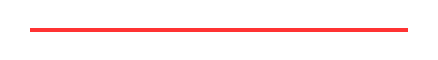
\begin{tikzpicture}
	\draw[red!80,ultra thick] (0,0) --(4.8,0);
	\end{tikzpicture}
	\end{textblock*}
\end{frame}
%--- Next Frame ---%

\begin{frame}[t]{연습문제}
	\begin{itemize}
	\item 두 명의 선수들($P1$, $P2$)이 있고 각각 0에서 100 사이의 정수를 적는다. 
	\item $a_1$이 선수1이 적어낸 수, $a_2$는 선수 2가 적어낸 수라고 하자. 
	\item 보수는 다음과 같은 룰에 따라서 결정된다. 
		\begin{enumerate}
		\item 만일 $a_1 + a_2 \leq 100$, 각각 $a_1$, $a_2$를 챙겨간다.
		\item 만일 $a_1 + a_2 > 100$ 이고 $a_1 > a_2$, $P1$은 $100-a_2$, $P2$는 $a_2$
		\item 만일 $a_1 + a_2 > 100$ 이고 $a_1 < a_2$, $P1$은 $a_1$, $P2$는 $100-a_1$
		\item 만일 $a_1 + a_2 > 100$ 이고 $a_1 = a_2$, $P1$과 $P2$는 모두 $50$
		\end{enumerate}
	\end{itemize}
	\begin{center}
	\framebox[20em]{이 게임의 ``균형''은 무엇인가?}
	\end{center}
\end{frame}
%--- Next Frame ---%

\begin{frame}[t]{약우월전략 (Weakly Dominant Strategy)}
	\begin{center}
	\begin{table}
	\setlength{\tabcolsep}{1.2em}
	\begin{tabular}{|c|c|c|c|} \hline
	& {L} &  {M} & {R}\\ \hline
	{U} & {$1$}, {$0$} & {$-2$}, {$-1$} & {$0$}, {$1$} \\ \hline%
	{D} & {$1$}, {$2$}  & {$-5$}, {$-1$} & {$0$}, {$0$} \\ 
	\hline
	\end{tabular}
	\end{table}
	\end{center}
	\vspace{1em}
	\begin{itemize}
		\item 어떤 순서에 따라 지우느냐에 따라서 균형이 달라짐
		\item 따라서 약우월전략에 따를 경우 균형 개념으로서의 효용은 떨어짐
	\end{itemize}
\end{frame}
%--- Next Frame ---%

% section equilibrium (end)

\section{Equilibrium} % (fold)
\label{sec:equilibrium}

\begin{frame}[t]{우월전략으로 균형을 찾는 방식의 문제점}
	\begin{columns}[c]
	\column{15em}
	\begin{itemize}
		\item 약弱우월전략이라면?
		\item (아예) 우월전략이 없다면?  
		\item 옆의 게임에서 우월 전략이 있는가? 
	\end{itemize}
	\column{15em}
	\begin{table}
	\setlength{\tabcolsep}{1.2em}
	\begin{tabular}{|c|c|c|c|} \hline
	& {L} &  {R}\\ \hline
	{L} & {$1$}, {$1$} & {$0$}, {$0$} \\ \hline%
	{R} & {$0$}, {$0$}  & {$2$}, {$2$}\\ 
	\hline
	\end{tabular}
	\end{table}
	\end{columns}
	\vspace{2em}
	\begin{center}
	\framebox[30em]{
	이럴 경우 우리는 이 게임의 결과를 어떤 기준에서 예측해야 하는가? 
	}
	\end{center}
\end{frame}
%--- Next Frame ---%

\begin{frame}[t]{Before Nash}
	\begin{itemize}
	\item von Neumann's concept of equilibrium
	\item 다음의 제로섬 게임을 살펴보자.\\
	\vspace{2em}
	\begin{center}
	\begin{table}
	\setlength{\tabcolsep}{1.2em}
	\begin{tabular}{|c|c|c|c|} \hline
	& {B1} &  {B2} & {B3}\\ \hline
	{A1} & {$3$} & {$-2$} & {$2$} \\ \hline%
	{A2} & {$-1$} & {$0$} & {$4$} \\ \hline
	{A3} & {$-4$}  & {$-3$} & {$1$} \\ \hline
	\end{tabular}
	\end{table}
	\end{center}
	\vspace{2em}
	\item 왜 보수를 하나만 썼을까? 
	\item 제로섬 게임의 특징을 고려해보자. 
	\end{itemize}
\end{frame}
%--- Next Frame ---%

\begin{frame}[t]{Minimax Theorem}
	\begin{itemize}
		\item 유한한 숫자의 전략을 지닌 두 명의 제로섬 게임에서 다음과 같은 $V$가 존재한다. 
		\begin{enumerate}
			\item 선수2의 전략이 주어졌을 때 선수 1의 가장 좋은 보수는 $V$이고, 
			\item 선수1의 전략이 주어졌을 때 선수 2의 가장 좋은 보수는 $-V$다. 
		\end{enumerate} 
	\end{itemize}
\end{frame}
%--- Next Frame ---%

\begin{frame}[t]{Minimax의 의미}
	\begin{itemize}
		\item 상대는 자기 보수의 최대화를 추구 (나의 입장에서는 최소화)
		\item 나도 내 보수의 최대화를 추구 (상대의 입장에서는 최대화)
		\item 나는 최소화된 내 보수의 최대화를 추구하는 것이 바람직
	\end{itemize}
\end{frame}
%--- Next Frame ---%

\begin{frame}[t]{Minimax Equilibrium}
	\begin{columns}
		\column{.5\textwidth}
		\begin{center}
			\begin{table}
			\begin{tabular}{|c|c|c|c|} \hline
			& {B1} &  {B2} & {B3}\\ \hline
			{A1} & {$3$} & {$-2$} & {$2$} \\ \hline%
			{A2} & {$-1$} & {$0$} & {$4$} \\ \hline
			{A3} & {$-4$}  & {$-3$} & {$1$} \\ \hline
			\end{tabular}
			\end{table}
		\end{center}
		\column{.5\textwidth}
		\begin{itemize}
			\item 균형: $(A2,B2)$
			\item 하지만 이 균형은 안정적일까? 
			\item 만일 선수1이 $A2$를 한다면 선수2는 $B1$으로 이탈하고자 할 것! 
			\item 따라서 안정적이지 않다!
			\item 균형은 존재여부 뿐만 아니라 안정성도 중요
		\end{itemize}
	\end{columns}
\end{frame}
%--- Next Frame ---%

\begin{frame}[t]{열등전략 지우기}
	\begin{columns}
		\column{.5\textwidth}
		\begin{center}
			\begin{table}
			\begin{tabular}{|c|c|c|c|} \hline
			& {B1} &  {B2} & {B3}\\ \hline
			{A1} & {$3$} & {$-2$} & {$2$} \\ \hline%
			{A2} & {$-1$} & {$0$} & {$4$} \\ \hline
			{A3} & {$-4$}  & {$-3$} & {$1$} \\ \hline
			\end{tabular}
			\end{table}
		\end{center}
		\column{.5\textwidth}
		\begin{itemize}
			\item 먼저 (강)열등전략을 지워보자. 
			\item 선수1에게는 $A3$,  선수2에게는?
			\item 전략을 확률적으로 쓸 수 있다고 해두자. 
			\item 즉, 두 개 혹은 그 이상의 전략을 확률적으로 내는 것이다. 
			\item 이렇게 되면 B의 어느 전략이 열등해질까?
		\end{itemize}
	\end{columns}
\end{frame}
%--- Next Frame ---%

\begin{frame}[t]{안정적인 전략 찾기}
	\begin{columns}
		\column{.4\textwidth}
		\begin{center}
			\begin{table}
			\begin{tabular}{|c|c|c|c|} \hline
			& {B1} &  {B2} & {B3}\\ \hline
			{A1} & {$3$} & {$-2$} & {$2$} \\ \hline%
			{A2} & {$-1$} & {$0$} & {$4$} \\ \hline
			{A3} & {$-4$}  & {$-3$} & {$1$} \\ \hline
			\end{tabular}
			\end{table}
		\end{center}
		\column{.6\textwidth}
		\begin{itemize}
			\item 이제 $A1, A2$ 그리고 $B1, B2$만 고려하도록 하자. 
			\item 선수1이 $A1$을 $p$의 확률로 $A2$를 $1-p$의 확률로 구사할 때 상대가 어떤 전략을 쓰더라도 둘의 결과가 동일해지는 경우를 찾아보고 선수2에 대해서도 비슷하게 답을 찾아보자. 
			\item 이러한 확률적인 대응은 안정적인가? 
			\\ 확인하는 방법은 이러한 전략적 대응에서 둘의 기대보수를 계산해보는 것.
		\end{itemize}
	\end{columns}
\end{frame}
%--- Next Frame ---%

% section equilibrium (end)

\section{Nash Equilibrium} % (fold)
\label{sec:nash_equilibrium}

\begin{frame}[t]{John Nash: 1928-2015}
	\begin{columns}[c]
	\column{18em}
	\begin{itemize}
		\item 보다 일반적인 균형의 개념을 찾아서 
		\item 일단 균형이 달성되었다고 가정한 후 
		\item 그 균형이 어떤 특징을 가져야 할지 상상해보기 
		\item 그리고 이러한 균형은 존재할까? 
	\end{itemize}
	\column{12em}
	\fbox{\includegraphics[width=11em]{johnnash.jpg}}
	\end{columns}
\end{frame}
%--- Next Frame ---%

\begin{frame}[t]{Nash Equilibrium: Main Idea}
	\begin{itemize}
		\item 일단 어떤 전략 조합 상태 (전략 프로파일)에 있다고 가정
		\item 이때 다른 선들이 그 상태에 머무르는 상황에서 선1만 전략을 바꿔 이득을 볼 수 있는가? 
		\begin{itemize}
			\item 만일 YES라면: 그 전략 프로파일은 균형이 아님 (why?)
			\item 만일 NO라면: 최소한 ``선1''은 전략을 바꾸지 않을 것임
		\end{itemize}
		\item 이런 식으로 나머지 모든 선들에 대해서 위 과정을 반복
		\item 만일 어떤 전략 프로파일이 모든 다른 선수들에 대해서도 모두 NO인 상태라면, 그 전략 프로파일이 바로 Nash Equilibrium (NE)
	\end{itemize}
\end{frame}
%--- Next Frame ---%

\begin{frame}[t]{Nash's Contribution}
	\begin{columns}[c]
	\column{18em}
	\begin{itemize}
		\item 균형 개념을 고안했다는 데에 있는 것이 아니라
		\item 유한한 수의 선수와 유한한 수의 전략이 있는 게임에서 
		\item (안정적인) 내시 균형이 반드시 하나 이상 존재한다는 점을 증명했다는 데에 있음
		\item 게임이 연구할 가치가 있는 대상임을 입증! 
	\end{itemize}
	\column{13em}
	\fbox{\includegraphics[width=11em]{pf.jpeg}}
	\end{columns}
\end{frame}
%--- Next Frame ---%

% section nash_equilibrium (end)

\section{Typical Games} % (fold)
\label{sec:typical_games}

\begin{frame}[t]{조정게임 (Coordination Game)}
	\begin{columns}[c]
		\column{18em}
		\begin{itemize}
			\item 선수들의 행동이 조정되어야 바람직한 상태에 도달 
			\item 사회의 표준, 관습의 중요성  
			\item 내시 균형은? 
		\end{itemize}
		\column{15em}
		\begin{table}
		\setlength{\tabcolsep}{1.2em}
		\begin{tabular}{|c|c|c|c|} \hline
		& {L} &  {R}\\ \hline
		{L} & {$1$}, {$1$} & {$0$}, {$0$} \\ \hline%
		{R} & {$0$}, {$0$}  & {$2$}, {$2$}\\ 
		\hline
		\end{tabular}
		\end{table}
	\end{columns}
\end{frame}
%--- Next Frame ---%

\begin{frame}[t]{순수전략 내쉬균형 (PSNE: Pure Strategy NE) 찾기}
	\begin{columns}
		\column{.4\textwidth}
			\begin{table}
			% \setlength{\tabcolsep}{1.2em}
			\begin{tabular}{|c|c|c|c|} \hline
			& {L} &  {R}\\ \hline
			{L} & {$1$}, {$1$} & {$0$}, {$0$} \\ \hline%
			{R} & {$0$}, {$0$}  & {$2$}, {$2$}\\ 
			\hline
			\end{tabular}
			\end{table}
		\column{.6\textwidth}
		\begin{enumerate}
			\item 전략의 모든 조합이 4개 밖에 안되니까 4개를 다 체크. 각각의 상태에서 다른 상태로 이탈할 때 선수 누구에게든 이득이 발생하는지 확인한다.\footnote{엄밀히는 곧 배우게 될 혼합전략까지 모두 고려해야 한다.}
			\item 각각의 플레이어에 대해서 상대의 행동이 내시 균형의 행동이라고 할 때 나의 행동은 어떤 것인지를 확인해준다. 이때 모든 사람의 행동이 이같은 원칙에 부합할 때 NE
		\end{enumerate}
	\end{columns}
\end{frame}
%--- Next Frame ---%

\begin{frame}[t]{최적 대응 (Best Response)}
	\begin{columns}
		\column{.4\textwidth}
			\begin{table}
			% \setlength{\tabcolsep}{1.2em}
			\begin{tabular}{|c|c|c|c|} \hline
			& {L} &  {R}\\ \hline
			{L} & {$1$}, {$1$} & {$0$}, {$0$} \\ \hline%
			{R} & {$0$}, {$0$}  & {$2$}, {$2$}\\ 
			\hline
			\end{tabular}
			\end{table}
		\column{.6\textwidth}
		\begin{enumerate}
			\item 두번째 방법은 최적 대응 (Best response)라고 한다. 
			\item 나에게 가장 이익이 되는 행위는 상대의 행동에 의존한다. 이때 상대의 행동/전략을 어떤 함수 혹은 관계의 $x$라고 할 때, 이 $x$에서 가장 최적의 대응을 만들어주는 전략 프로파일이 NE
			\item 앞서의 예에서 $B_1(L)=L$, $B_1(R)=R$과 같이 나타낼 수 있다.
		\end{enumerate}
	\end{columns}
\end{frame}
%--- Next Frame ---%

\begin{frame}[t]{매-비둘기 게임 (= 겁쟁이 게임)}
	\begin{columns}[c]
	\column{18em}
	\begin{itemize}
		\item 조정 게임과는 반대의 상황  
		\item 다른 이름: Chicken game, snow-drift game 
	\end{itemize}
	\column{15em}
	\begin{table}
	\setlength{\tabcolsep}{1.2em}
	\begin{tabular}{|c|c|c|c|} \hline
	& {H} &  {D}\\ \hline
	{H} & {$-\frac{1}{2}$}, {$-\frac{1}{2}$} & {$1$}, {$0$} \\ \hline%
	{D} & {$0$}, {$1$}  & {$\frac{1}{2}$}, {$\frac{1}{2}$}\\ 
	\hline
	\end{tabular}
	\end{table}
	\end{columns}
\end{frame}
%--- Next Frame ---%

\begin{frame}[t]{죄수의 딜레마 (Prisoner's Dilemma) 게임}
	\begin{columns}[c]
	\column{18em}
	\begin{itemize}
		\item 이미 우리가 살펴본 게임 
		\item 우월 전략이 존재하고, 이는 PSNE과 동일  
	\end{itemize}
	\column{15em}
	\begin{table}
	\setlength{\tabcolsep}{1.2em}
	\begin{tabular}{|c|c|c|c|} \hline
	& {C} &  {D}\\ \hline
	{C} & {$2$}, {$2$} & {$0$}, {$3$} \\ \hline%
	{D} & {$3$}, {$0$}  & {$1$}, {$1$}\\ 
	\hline
	\end{tabular}
	\end{table}
	\end{columns}
\end{frame}
%--- Next Frame ---%

\begin{frame}\frametitle{Matching Pennies}\vspace{3em}
	\begin{columns}[c]
		\column{18em}
		\begin{itemize}
		\item 간단한 버전의 짤짤이 
		\item 선수1이 백원짜리 동전의 앞뒤를 접고, 선수2가 맞춘다. 
		\item 이 게임의 내시 균형은 있는가? 
		\end{itemize}
		\column{15em}
		\begin{table}
		\setlength{\tabcolsep}{1.2em}
		\begin{tabular}{|c|c|c|c|} \hline
		& {H} &  {T}\\ \hline
		{H} & {$-1$}, {$1$} & {$1$}, {$-1$} \\ \hline%
		{T} & {$1$}, {$-1$}  & {$-1$}, {$1$}\\ 
		\hline
		\end{tabular}
		\end{table}
	\end{columns}
\end{frame}

\begin{frame}[t]{혼합전략 (Mixed Strategy)}
	\begin{columns}[c]
	\column{18em}
	\begin{itemize}
		\item 분명 Nash는 모든 게임에 균형이 있다고 했는데??
		\item 과연 이 문제를 어떻게 해결할 것인가? 
		\item 앞서 ZSG (Zero Sum Game) 의 사례를 기억하는가? 
		\item Nash가 염두한 전략은 전략들을 확률적으로 구사하는 것: 혼합전략
	\end{itemize}
	\column{13em}
	\fbox{\includegraphics[width=12em]{rsc.png}}
	\end{columns}
	\end{frame}

	\begin{frame}{How to Find MSNE}
	\begin{itemize}
	\item $P1$은 $H$를 $p$의 확률로, $P2$는 $H$를 $q$의 확률로 구사
	\item 각각의 페이오프를 식으로 적어보면
	\begin{align*}
	\pi_1 &= pq[-1]+p(1-q)[1]+(1-p)q[1]+(1-p)(1-q)[-1] \\
	         &=p(1-2q)-(1-p)(1-2q) \\
	         &=(1-2q)(2p-1)
	\end{align*}
	\item 마찬가지로 구해보면 $\pi_2$? 
	\item 앞서 배웠던 최적 대응의 개념을 여기에 적용해보자
	\end{itemize}
\end{frame}
%--- Next Frame ---%

\begin{frame}[t]{MSNE를 찾는 좀 더 쉬운 방법}
	\begin{itemize}
		\item 혼합전략 아래에서는 플레이어는 어떤 전략을 구사하더라도 동일한 보수를 얻어야 한다. 이를 이용하면 쉽게 $p$, $q$를 찾을 수 있다. 
		\item 즉, 서로가 혼합전략을 구사한다고 하자. 이때 $P1$이 $H$와 $T$를 통해 얻는 보수는 각각 다음과 같다. 
		\begin{align*}
			\pi_1 (H)&= q [-1] + (1-q) [1] \\
			\pi_1 (T)&= q [1] + (1-q) [-1] 
		\end{align*}
		\item $P1$에게 이 두 값이 같을 때에만, $\pi_1(H)=\pi_1(T)$, $P1$은 혼합전략을 구사하게 될 것이다. 만일 다르다면 당연히 100\%의 확률로 보수가 더 높은 전략을 구사할 것이다. 
		\item 따라서, $P2$의 최적의 전략은 $q^*=\frac{1}{2}$. 마찬가지로 $p^*=\frac{1}{2}$. 
	\end{itemize}
\end{frame}
%--- Next Frame ---%

% section typical_games (end)

\end{document}